\documentclass[a4paper,12pt]{article}
\usepackage[utf8]{inputenc}
\usepackage[english,russian]{babel}
\usepackage[T2A]{fontenc}
\usepackage{mathtext}
\usepackage{gauss}
\usepackage{graphicx}
\usepackage{amsmath, amsfonts, amssymb}
\newtheorem{theorem}{Теорема}
\usepackage[left=2.50cm, right=2.00cm, top=2.00cm, bottom=2.00cm]{geometry} 
\usepackage{mathdots} 
\usepackage[pdftex]{lscape}
\usepackage{mathtools}
\usepackage{pgfplots}
\pgfplotsset{compat=1.9}
\usepackage{graphicx}%Вставка картинок правильная
\usepackage{tikz}
\usepackage{float}%"Плавающие" картинки
 \usepackage{relsize}
\usepackage{wrapfig}%Обтекание фигур (таблиц, картинок и прочего)
\usepackage{ tipa }
\usepackage{amsmath}
  \usepackage[unicode=true, colorlinks=true, linkcolor=blue, urlcolor=blue]{hyperref}
\linespread{1}
\newcommand{\om}{\overline{o}}
\newcommand{\OB}{\underline{O}}
\newcommand{\eps}{\varepsilon}
\newcommand{\RR}{\mathbb{R}}
\newcommand{\NN}{\mathbb{N}}
\newcommand{\CC}{\mathbb{C}}
\newcommand{\QQ}{\mathbb{Q}}
\newcommand{\ZZ}{\mathbb{Z}}
\newcommand{\dx}{\d{dx}}
\newcommand{\ph}{\varphi}
\newcommand{\F}{\mathbb{F}}
\newcommand{\E}{\mathbb{E}}
\begin{document}
	\section*{1}
	\subsection*{a)}
	$$f(x) = \begin{cases}
		2^{x^{-1}},x\ne0\\
	-3,x = 0	\end{cases}$$
	$$\lim_{x\to 0+0}\left\{2^{x^{-1}}\right\} = \infty$$
	$$\lim_{x\to 0-0}\left\{2^{x^{-1}}\right\} = 0$$
	f(0) = -3 $\to $ 0- точка разрыва третьего рода
	\begin{figure}[h]
		\centering
		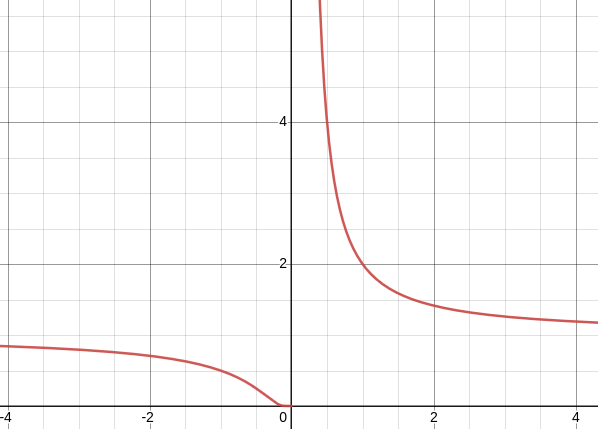
\includegraphics[width=0.8\linewidth]{Screenshot from 2023-11-24 11-38-33.png}
		\label{fig:mpr}
	\end{figure}
	\subsection*{b)}
	$$f(x)= \begin{cases}
	\arctan{\frac1x}\quad x\ne0 \\
	0,\quad x=0	\end{cases}$$
		$$\lim_{x\to 0+0}f(x) = \pi/2$$
	$$\lim_{x\to 0-0}f(x) = -\pi/2$$ $\to $ точка разрыва первого рода
		\begin{figure}[h]
		\centering
		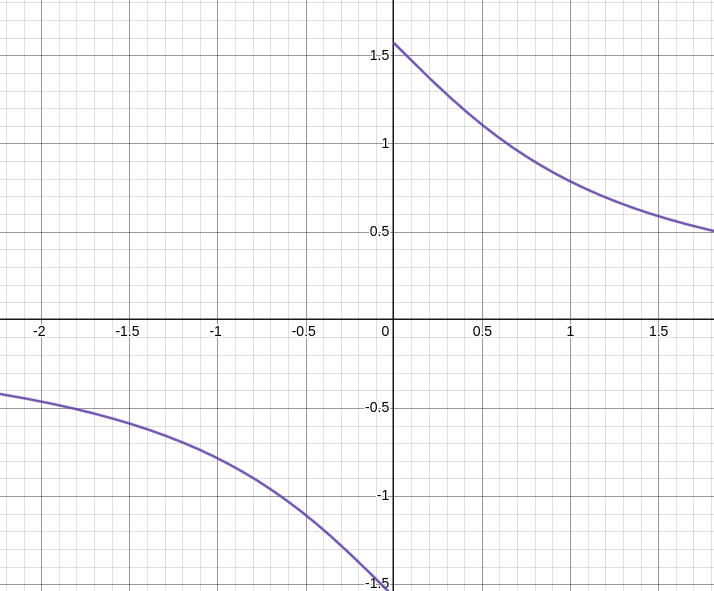
\includegraphics[width=0.8\linewidth]{Screenshot from 2023-11-24 11-51-25.png}
		\label{fig:mpr}
	\end{figure}
	\subsection*{c)}
	$$f(x) = \begin{cases}
	x, x\in \QQ\\ 
	x, x\in\RR\backslash\QQ\end{cases}$$
	$$\lim_{x\to 0+0} f{x}=0 $$
	$$\lim_{x\to 0-0} f{x}=0 $$
	$$f(x) = 0\to \text{Ноль- не точка разрыва.}$$
	Во всех остальных вещественных точках разрыв нулевого рода, т.к функция в окрестности этих точек близко приближается к вещественному значени, но никогда не равняется ему.	
	\section*{2}
	$$\lim_{x\to 0+0}\frac{\cos{\sin{3x}}}{x^2} = \lim_{x\to 0+0}\frac{\cos{3x+\om(x)}}{x^2} = \frac{1-\frac92x^2-1}{x^2} = \frac92$$
		$$\lim_{x\to 0-0}\frac{\cos{\sin{3x}}}{x^2} = \lim_{x\to 0-0}\frac{\cos{3x+\om(x)}}{x^2} = \frac{1-\frac92x^2-1}{x^2} = \frac92$$
	Если $\lambda =\frac92$, то функция непрерывна в точке 0.
	\section*{3}
	\subsection*{a)}
	$$y=\frac{2+x^2}{\sqrt{1+x^4}}$$
	$$y^{'} =\frac{2x(\sqrt{1+x^4})-(2+x^2)\cdot\frac{4x^3}{2\sqrt{1+x^4}}}{1+x^4} =\frac{2x-4x^3}{(1+x^4)\sqrt{1+x^4}}$$
	\subsection*{b)}
	$$(\arcsin{5^{x^2}})^{'} = (\arcsin\circ\quad5x^2)^{'} = \frac{5^{x^2}\cdot\ln5\cdot2x}{\sqrt{1-5^{x^2}}}$$
	\subsection*{c)}
	$$f(x) = \left(2 + \cos{3x}\right)^{\ln x}$$
	$$f^{'}(x) = (2+\cos{3x})^{\ln x}\cdot\left(\frac1x\cdot\ln(2+\cos3x)-f\frac{3\ln x\cdot\sin 3x}{2+\cos3x}\right)$$
	\subsection*{d)}
    $$f(x) = 2^{\arctan{\sqrt{1+x^2}}}$$
    $$(\arctan{\sqrt{1+x^2})^{'} = \frac{1}{\sqrt{1+x^2}^2+1}\cdot\frac{1}{2\sqrt{1+x^2}}\cdot2x} = \frac{2x}{(2+x^2)\sqrt{1+x^2}}$$
    $$f^{'}(x) =2^{\arctan{\sqrt{1+x^2}}}\cdot\left(\frac{2x}{(2+x^2)\sqrt{1+x^2}}\right) $$
    \subsection*{e)}
    $$f(x) = x^{a^a} + a^{x^a} + a^{a^x}$$
    $$(x^{a^a})^{'} = x^{a^a-1}$$
    $$(a^{x^a})^{'} = a^{x^a}\cdot \ln{a}\cdot a\cdot x^{a-1}$$
    $$a^{a^x} = (a^x\circ a^x) = a^{a^x}\cdot\ln(a)\cdot\ln(a)\cdot a^x = ln^2(a)\cdot a^{a^x+x}$$
    $$f^{'}(x) =x^{a^a-1} +  a^{x^a}\cdot \ln{a}\cdot a\cdot x^{a-1} + ln^2(a)\cdot a^{a^x+x}$$
    \section*{4}
    $$f(x) = \begin{cases}
    	x^2\cdot\sin{\frac1x} ,\quad x\ne 0\\
    	0, \quad x=0
    \end{cases}$$
        $$f^{'}(x) = \begin{cases}
    	2x\sin{\frac1x}-\cos{\frac1x} ,\quad x\ne 0\\
    	\lim_{\delta\to 0}\frac{f(0+\delta)-f(0)}{\delta}, \quad x=0
    \end{cases}$$
    $$	\lim_{\delta\to 0}\frac{f(0+\delta)-f(0)}{\delta} = \frac{\delta^2\cdot\sin{\frac1\delta}}{\delta} = \delta\sin{\frac1\delta}= 0$$
            $$f^{'}(x) = \begin{cases}
    	2x\sin{\frac1x}-\cos{\frac1x} ,\quad x\ne 0\\
    	0, \quad x=0
    \end{cases}$$
\end{document}